% gOMSguide.tex
% v5.0 released July 2015

\documentclass{gOMS2e}

\usepackage{epstopdf}% To incorporate .eps illustrations using PDFLaTeX, etc.
\usepackage{subfigure}% Support for small, `sub' figures and tables

\theoremstyle{plain}% Theorem-like structures
\newtheorem{theorem}{Theorem}[section]
\newtheorem{corollary}[theorem]{Corollary}
\newtheorem{lemma}[theorem]{Lemma}
\newtheorem{proposition}[theorem]{Proposition}

\theoremstyle{definition}
\newtheorem{definition}{Definition}

\theoremstyle{remark}
\newtheorem{remark}{Remark}

\begin{document}

%\jvol{00} \jnum{00} \jyear{2015} \jmonth{July}

%\articletype{GUIDE}

\title{GLOBALIZER: A NOVEL SUPERCOMPUTER SOFTWARE SYSTEM FOR SOLVING TIME-CONSUMING GLOBAL OPTIMIZATION PROBLEMS}

\author{
\name{V. P. Gergel\textsuperscript{a}$^{\ast}$\thanks{$^\ast$Corresponding author. Email: gergel@unn.ru}
and K. A. Barkalov\textsuperscript{b} and A. V. Sysoev}
\affil{\textsuperscript{a}Taylor \& Francis, 4 Park Square, Milton Park, Abingdon, UK;
\textsuperscript{b}State University of Nizhny Novgorod, Nizhny Novgorod, Russia}
}

\maketitle

\begin{abstract}
In this paper, we describe the Globalizer software system for solving global optimization
problems. The system is designed to maximize the use of computational potential by modern
high performance computer systems in order to solve the most time-consuming optimization
problems. Highly parallel computations are facilitated using various distinctive computational
schemes: processing several optimization iterations simultaneously, reducing multidimensional
optimization problems using multiple Peano curve evolvents, multi-stage computing based on
nested block reduction schemes. This novelty leverages supercomputer system capabilities
with shared and distributed memory and with large numbers of processors to efficiently
solve global optimization problems.
\end{abstract}

\begin{keywords}
global optimization, information-statistical theory, parallel computing, high-performance
computer systems, supercomputer technologies
\end{keywords}

\section{Introduction}
\label{sec:intro}
Global (or multiextremal) optimization problems are among the most complex problems
in both theory and practice for optimal decision making. In these kinds of problems,
the criterion to be optimized has several local optima within the search domain,
which have different values. The existence of several local optima essentially makes
finding the global optimum difficult, since it requires examining the whole feasible
search domain. The volume of computations for solving global optimization problems
can increase exponentially with increasing number of varied parameters.
\par
In addition, global optimization problem statements are used, as a rule, in the most
complex decision making situations, for example, when a computer-aided design of complex
technologies, products, and systems is conducted. In such problems, the efficiency
criteria are nonlinear, the search domains may be non-contiguous, and, most importantly,
the computational complexity of the functions which the optimized criteria and constraints
are based on can be quite essential.
\par
These global optimization problem features impose special requirements on the quality of
the optimization methods and on the software to implement them. The global optimization
methods should be highly efficient, and the software systems should be developed on a good
professional basis. In general, global optimization problems can be solved using modern
supercomputer systems at a reasonable time and cost by only employing parallel
global optimization algorithms.
\par
The general state of the art in the field of global optimization has been presented in a
number of key monographs (Törn, A., Žilinskas, A., 1989), (Horst, R., Tuy, H., 1990), (Zhigljavsky, A. A., 1991), (Pintér, J. D., 1996), (Strongin, R. G., Sergeyev, Y. D., 2000), (Locatelli, M., Schoen, F., 2013), (Floudas, C. A., Pardalos, M. P., 2016), etc.
The development of optimization methods that use high-performance computer systems to
solve time-consuming global optimization problems is an area receiving extensive
attention – see, for example, (Censor, Y., Zenios, S. A., 1998), (Strongin, R. G., Sergeyev, Y. D., 2000), (Ciegis, R., Henty, D., Kågström, B., Zilinskas, J., 2009), (Luque, G., Alba, E., 2011), (Strongin, R. G., K. A., Gergel, V. P., Grishagin, V. A., Barkalov, K. A.,  2013).
\par
The theoretical results obtained provide efficient solutions to many applied global
optimization problems in various fields of scientific and technological applications – see,
for example, (Floudas, C. A., Pardalos, M. P., 1996), (Pintér, J. D., 1996), (Luque, G., Alba, E., 2011), (Fasano, G., Pintér, J. D., (2013), (Locatelli, M., Schoen, F., 2013), (Pardalos, M. P., Zhigljavsky, A. A., Zilinskas, J., 2016), etc.
\par
At the same time, the practical implementation of these algorithms for multiextremal
optimization within the framework of industrial software systems is quite limited.
In many cases, software implementations of global optimization algorithms are experimental in
nature and are just used by the developers themselves to obtain results from computational
experiments required for scientific publication. To a large extent, this situation
originates from high development costs for professional software systems that can be
used by numerous users. In addition, global optimization problems could rarely be
solved in an automatic mode because of their complexity. As a rule, the user should
actively control the global search process which implies an adequate level of
qualification in the field of optimization (particularly, the user should know and
understand global optimization methods well).
\par
On the market for global optimization software, one can select from the following systems:
\begin{itemize}
\item LGO (Lipschitz Global Optimization) is designed to solve global optimization
problems for which the criteria and constraints satisfy the Lipschitz condition (see, for example, (Pintér, J. D., 1996)).
The system is a commercial product based on diagonal extensions of one-dimensional
multiextremal optimization algorithms.
\item GlobSol (Kearfott, R. B., 2009) is oriented towards solving global optimization problems as well as
systems of nonlinear equations. The system includes interval methods based on the branch and
bound method. There are some extensions of the system for parallel computations, and it is available to use for free.
\item LINDO (Lin, Y., Schrage.L., 2009) is features by a wide spectrum of problem solving mehtods which
it can be used for – these include linear, integer, stochastic, nonlinear, and global
optimization problems. The ability to interact with the Microsoft Excel software
environment is a key feature of the system. The system is widely used in practical
applications and is available to use for free.
\item IOSO (Indirect Optimization on the basis of Self-Organization) is oriented
toward solving of a wide class of the extremal problems including global optimization
problems (see, for example, (Egorov, I. N., Kretinin, G. V., Leshchenko, I. A., Kuptzov, S. V., 2002)). The system is widely used to
solve applied problems in various fields. There are versions of the system for parallel
computational systems. The system is a commercial product, but is available for trial use.
\item MATLAB Global Optimization Toolkit (see, for example, (Venkataraman, P., 2009)) includes a wide spectrum
of methods for solving the global optimization problems, including multistart methods,
global pattern search, simulated annealing methods, etc. The library is compatible to the
TOMLAB system (see, for example, (Holmström, K., Edvall, M. M., 2004)), which is an additional extension the widely-used MATLAB.
It is also worth noting that similar libraries for solving global optimization problems are
available for MathCAD, Mathematica, and Maple systems as well.
\item BARON (Branch-And-Reduce Optimization Navigator) is designed to solve continuous
integer programming and global optimization problems using the branch and bound method (Sahinidis, N. V., 1996).
BARON is included in the GAMS (General Algebraic Modeling System) system used extensively – see (Bussieck, M. R., Meeraus, A., 2004).
\item Global Optimization Library in R is a large collection of optimization methods
implemented in the R language (see, for example, (Mullen, K. M., 2014)). Among these methods, are stochastic and deterministic global optimization algorithms,
the branch and bound method, etc.
\end{itemize}
\par
The list provided above is certainly not exhaustive – additional information on software
systems for a wider spectrum of optimization problems can be obtained, for example,
in (Rios, L. M., Sahinidis, N. V., 2013), (Mongeau, M.,  Karsenty, H., Rouzé, V., Hiriart-Urruty, J. B., 2000), (Pintér, J. D., 2009), etc.
Nevertheless, even from such a short list the following conclusions can be drawn (see also Liberti, L., 2006):
\begin{itemize}
\item  the collection of available global optimization software systems for practical use is insufficient,
\item the availability of numerous methods through these systems allows complex
optimization problems to be solved in a number of cases, however, it requires a rather
high level of user knowledge and understanding in the field of global optimization,
\item the use of the parallel computing to increase the efficiency in solving complex
time-consuming problems is limited, therefore, the computational potential of modern
supercomputer systems is very poorly utilized.
\end{itemize}
\par
In this paper, a novel Globalizer software system is considered. The development of the
system was conducted based on the information-statistical theory of multiextremal
optimization aimed at developing efficient parallel algorithms for global search – see, for example, (Strongin, R. G., 1978), (Strongin, R. G., Sergeyev, Y. D., 2000), (Strongin, R. G., K. A., Gergel, V. P., Grishagin, V. A., Barkalov, K. A., 2013).
The advantage of the Globalizer is that the system is designed to solve time-consuming
multiextremal optimization problems. In order to obtain global optimized solutions
within a reasonable time and cost, the system efficiently uses modern high-performance computer systems.
\par
This paper is further structured as follows. In Section \ref{sec:problem}, a statement of the multidimensional
global optimization problem is presented, and an approach to reducing these to one-dimensional
optimization problems is described. In Section \ref{sec:parallel}, parallel computation schemes are presented,
and parallel optimization methods are described. In Section \ref{sec:arch}, the Globalizer architecture
is examined. In Section \ref{sec:experiments}, the results are presented from computational experiments
that confirm the system’s high level of efficiency. Finally, Section \ref{sec:concl} presents the
conclusions and some ideas for future research.

\section{Multidimensional Global Optimization Problems and Dimension Reduction}
\label{sec:problem}
In this paper, the core class\footnote{In general, the Globalizer can be applied for solving
multicriterial multiextremal multidimensional optimization problems with nonlinear constraints.} of
optimization problems which can be solved using the
Globalizer is examined. This involves multidimensional global optimization problems
without constraints, which can be defined in the following way:
\begin{equation}
\label{eq:task}
\begin{array}{cr}\\
  \varphi(y^*)=\min\{\varphi(y):y\in D\} \\
  D=\{y\in \mathbf{R}^N:a_i\leqslant x_i\leqslant{b_i}, 1\leqslant{i}\leqslant{N}\}
\end{array}
\end{equation}
where the objective function (y) satisfies the Lipschitz condition
\begin{equation}
\label{eq:lip}
|\varphi(y_1)-\varphi(y_2)|\leqslant L\Vert y_1-y_2\Vert,y_1,y_2\in D,
\end{equation}
where \(L>0\) is the Lipschitz constant, and \(||*||\) denotes the norm in \(\mathbf{R}^N\) space.
\par
Let us further assume that the minimized function \(\varphi(y)\) is defined as a
computational procedure, according to which the value \(\varphi(y)\) can be calculated
for any value of vector \(y\in D\) (let us further call the process of obtaining a
value for the minimized function a trial). As a rule, this procedure is computational-costly i.e.
the overall costs of solving optimization problem (\ref{eq:task}) are determined,
first of all, by the number of trials executed. It is also worth noting the essence of the
assumption on satisfying the Lipschitz condition, since one can construct an estimate
of the global minimum based on a finite number of computed values from the optimized function in this case only.
\par
As has been previously shown by many researchers, finding numerical estimates of globally
optimal extrema implies constructing coverage of the search domain \(D\). As a result,
the computational costs of solving global optimization problems are already very high
even for a small number of varied parameters (the dimensionality of the problem).
A notable reduction in the volume of computations can be achieved when the coverages of the
search domain being obtained are non-uniform, i.e. the series of trial points is dense
only in terms of its nearness to the sought-after globally optimized variants.
The generation of such non-uniform coverages could only be provided in an adaptive
way when the selection of the next trial points is determined by the search information
(the preceding trial points and the values of the minimized function at these points)
obtained in the course of computation. This necessary condition considerably
complicates the computational schemes for global optimization methods, since it
implies a complex analysis of a large amount of multidimensional search information.
As a result, many optimization algorithms use, to some extent, various methods of dimensional reduction.
\par
Within the framework of the information-statistical approach, Peano curves (or evolvents)
\(y(x)\) mapping the interval \([0, 1]\) onto an \(N\)-dimensional hypercube \(D\) are
unambiguously used for dimensional reduction (see, for example, Strongin, R. G., Sergeyev, Y. D., 2000).
\par
As a result of the reduction, the initial multidimensional global optimization
problem (\ref{eq:task}) is reduced to the following one-dimensional problem:
\begin{equation}
\label{eq:oneDimTask}
\varphi(y(x^*))=\min\{\varphi(y(x)):x\in [0,1]\}
\end{equation}
\par
The dimensional reduction scheme considered above superimposes a multidimensional
problem with a minimized Lipschitz function to a one-dimensional problem with a
corresponding minimized function to satisfy the uniform Hölder condition (see Strongin, R. G., 1978, Strongin, R. G., Sergeyev, Y. D., 2000) i.e.
\begin{equation}
\label{eq:holder}
|\varphi(y(x_1))-\varphi(y(x_2))|\leqslant H{|x_1-x_2|}^{\frac{1}{N}},x_1,x_2\in[0,1]
\end{equation}
where the constant \(H\) is defined by the relationship \(H=4L\sqrt{N}\), \(L\) is the
Lipschitz constant from (\ref{eq:lip}), and \(N\) is the dimensionality of the optimization problem (\ref{eq:task}).
\par
The algorithms for the numerical construction of the Peano curve approximations are presented in (Strongin, R. G., Sergeyev, Y. D., 2000).
As an illustration, an approximation of a Peano curve for the third level of density is
shown in Figure \ref{fig:peanoC}. The curve shown in Figure \ref{fig:peanoC} demonstrates the winding order of a
two-dimensional domain; the precision of the Peano curve approximation is determined by the
level of density used in the construction.

\begin{figure}[h!]
    \centering
		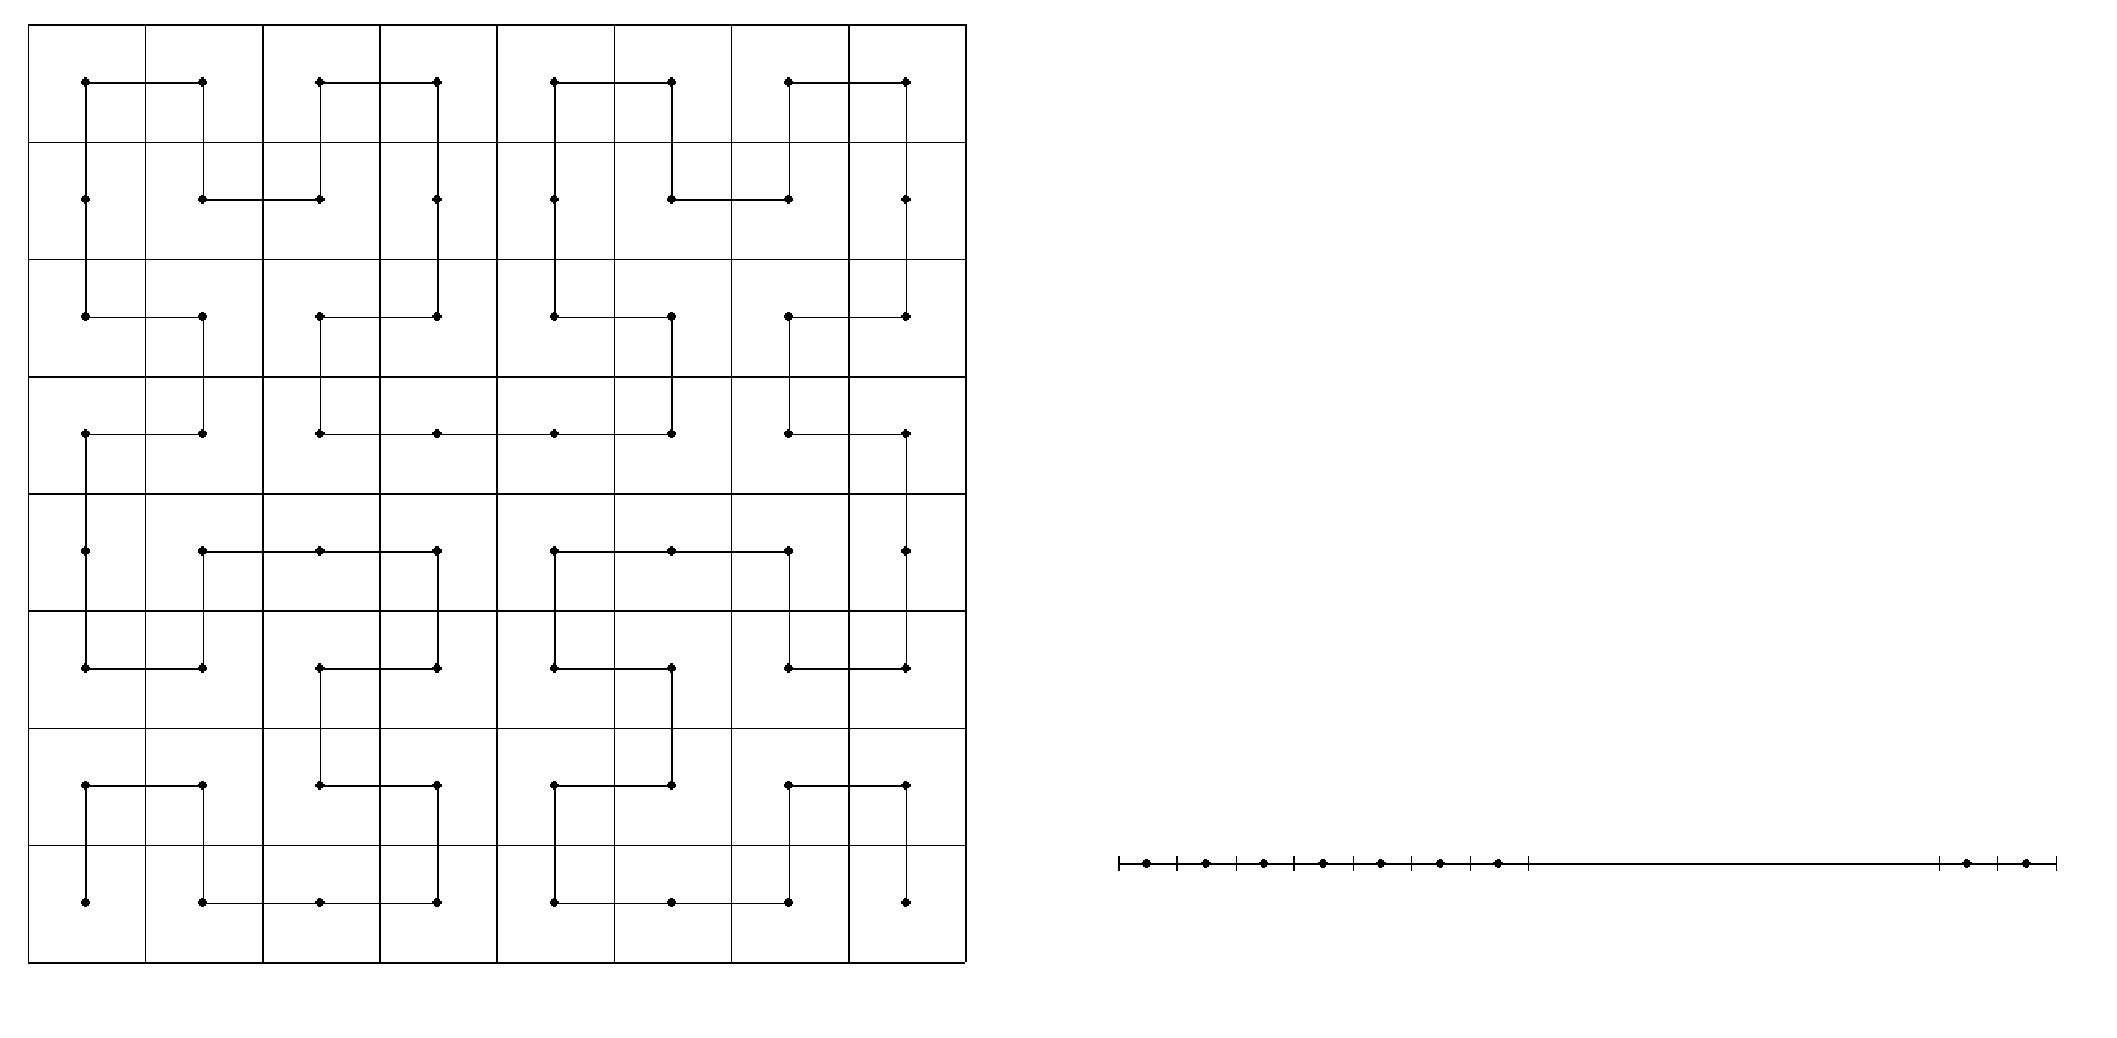
\includegraphics[width=0.85\textwidth]{pictures/peanoC.eps}
		\caption{A Peano curve approximation for the third level of}
    \label{fig:peanoC}
\end{figure}

\par
The computational scheme obtained as a result of the dimensional reduction consists of the following (see Figure \ref{fig:peanoCUsage}):
\begin{itemize}
  \item The optimization algorithm performs the minimization of the reduced one-dimensional function \(\varphi(y(x)\),
  \item After determining the next trial point \(x\), a multidimensional image \(у\) in the mapping \(y(x)\) is calculated,
  \item The value of the initial multidimensional function \(\varphi(y)\) is calculated at the multidimensional point \(у\in D\),
  \item The calculated value \(z=\varphi(y)\) is used further as the value of the reduced one-dimensional function \(\varphi(y(x))\) at the point \(x\).
\end{itemize}

\begin{figure}[h!]
    \centering
		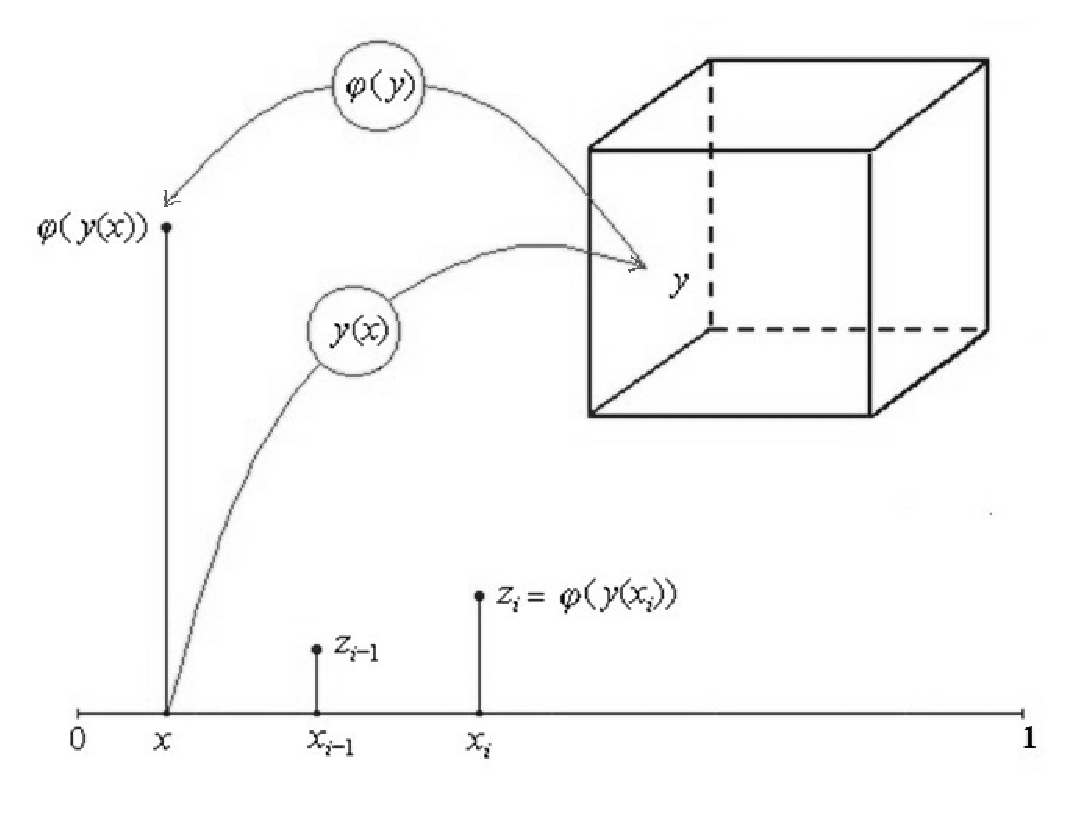
\includegraphics[width=0.55\textwidth]{pictures/peanoCUsage.eps}
		\caption{The computational scheme for obtaining the value of the reduced one-dimensional function \(\varphi(y(x))\)}
    \label{fig:peanoCUsage}
\end{figure}

\section{The Parallelization Approach and Global Optimization Algorithms}
\label{sec:parallel}
Let us consider the parallelization methods used widely in the theoretical and
practical application of parallel computing within the context of global optimization problems:
\begin{itemize}
  \item The distribution of the search domain \(D\) among the available computing units
  (data parallelization scheme). In the case of optimization problems, this approach is
  insufficient, since in organizing such computations the subdomain, which contain the
  sought global minimum, will be processed by only one processor, and, therefore,
  all of the remaining processors would perform the excess computations.
  \item The parallelization of the computational schemes for optimization algorithms
  (task parallelization scheme). This approach is also insufficient since the direct
  computational costs for executing optimization algorithms are relatively low
  (the majority of computations in the course of a global search are represented by
  calculations of the optimized function values due to the initial assumption of
  considerable computational costs for such calculations).
  \item The parallelization of the computations executed in order to obtain values
  for the optimized function. This approach can be applied since the most computationally
  costly part of the global search process will be parallelized. However, this method is not
  featured by the generality (the development of parallelization methods is to be performed
  every time from scratch while solving each particular optimization problem).
\end{itemize}
\par
Within the framework of information-statistical theory, a general approach to
parallelization computations when solving global optimization problems has been
proposed --- \textit{the parallelism of computations is provided by means of simultaneously
computing the values of the minimized function \(\varphi(y)\) at several different
points within the search domain \(D\)} – see, for example, (Strongin, R. G., Sergeyev, Y. D., 2000), (Strongin, R. G., K. A., Gergel, V. P., Grishagin, V. A., Barkalov, K. A.,  2013).
This approach provides parallelizaion for the most costly part of computations in the global search process.
\par
The global optimization algorithms implemented in Globalizer will be described step-by-step below.
In Subsection \ref{subsec:corepar}, the core sequential multidimensional algorithm of global search (MAGS) will be presented.
In Subsection \ref{subsec:sharedpar}, a parallel generalization of the MAGS algorithm for parallel computations on
computer systems with shared memory will be described. In Subsection \ref{subsec:distribpar}, the scheme
for parallel computations by multiprocessor systems with distributed memory will be provided.

\subsection{Core Multidimensional Generalized Algorithm of Global Search}
\label{subsec:corepar}
The information-statistical theory of global search formulated in (Strongin, R. G., 1978), (Strongin, R. G., Sergeyev, Y. D., 2000)
has served as a basis for the development of a large number of efficient multiextremal
optimization methods --- see, for example, (Gergel, V. P., 1996, 1997), (Gergel, V. P., Strongin, R. G., 2003, 2005), (Grishagin, V. A., Strongin, R. G., 1984), (Sergeyev Y. D., 1995, 1999), (Sergeyev, Y. D., Grishagin V. A., 1994, 2001), (Sergeyev, Y. D., Strongin, R. G., Lera, D., 2013), (Barkalov K. A., Gergel V. P., 2014), etc.
\par
Multidimensional Algorithm of Global Search (MAGS) established the basis for the
methods applied in Globalizer. The general computational scheme of MAGS can be
presented as follows --- see (Strongin, R. G., 1978), (Strongin, R. G., Sergeyev, Y. D., 2000).
\par
Let us introduce a simpler notation for the problem being solved on a computing node
\begin{equation}
\label{eq:oneDimFunc}
f(x) = \varphi(y(x)):x\in [0,1]\}
\end{equation}
\par
The initial iteration of the algorithm is performed at an arbitrary point \(x^1(0,1)\).
Let us assume further \(k\), \(k>1\), iterations of a global search are to be completed.
The selection of the trial point \(k+1\) for the next iteration is performed according to the following rules.
\par
\textit{Rule 1}. To renumber the points for the preceding trials by the lower indices in order of increasing value of coordinates
\begin{equation}
  \label{step1}
0=x_0<x_1<\dotsc<x_{k+1}=1
\end{equation}
the points \(x_0\), \(x_k\) were introduced additionally for convenience in further explanation,
the values of the minimized function \(z_0\), \(z_k\) at these points are undefined.
\par
\textit{Rule 2}. To compute a current estimate of the Hölder constant \(H\) from (\ref{eq:holder})
\begin{equation}
  \label{step2}
m=\max_{1\leqslant i\leqslant k}\dfrac{|z_i-z_{i-1}|}{\rho_i},
\begin{matrix}
    M =
    \left\{
    \begin{matrix}
    r\cdot u,m>0 \\
    1,m=0
    \end{matrix} \right.
    \end{matrix}
\end{equation}
as the maximum of the relative differences of the minimized function \(f(x)\) from (\ref{eq:oneDimFunc})
on the set of executed trial points \(x_i,1\leqslant i\leqslant k\) from (\ref{step1}). Further, \(\rho_i=(x_i-x_{i-1})^\frac{1}{N},1\leqslant i\leqslant k+1\).
The constant \(r\), \(r>1\), is the \textit{parameter} for the algorithm.
\par
\textit{Rule 3.} For each interval \((x_{i-1},x_i),1\leqslant i\leqslant k+1\), compute the characteristics \(R(i)\) where
\begin{equation}
\label{step3}
\begin{array}{cr}\\
  R(i)=\rho_i+\dfrac{(z_i-z_{i-1})^2}{M^2\rho_i}-2\dfrac{z_i+z_{i-1}}{M},\quad 1<i<k+1 \\
  R(i)=2\rho_1-4\dfrac{z_1}{M},\quad i=1 \\
  R(i)=2\rho_{k+1}-4\dfrac{z_k}{M},\quad i=k+1
\end{array}
\end{equation}
\par
\textit{Rule 4.} To determine the interval with the maximum characteristic
\begin{equation}
\label{step4}
R(t)=\max_{1\leqslant i \leqslant k+1}R(i)
\end{equation}
\par
\textit{Rule 5.} To execute a new trial (computation of the minimized function value \(f(x)\))
at the point \(x^{k+1}\) located within the interval with the maximum characteristic from (\ref{step4})
\begin{equation}
\label{step5}
\begin{array}{cr}\\
  x_{k+1}=\dfrac{x_t+x_{t-1}}{2}-sign(z_{t}-z_{t-1})\dfrac{1}{2r}\left[\dfrac{|z_{t}-z_{t-1}|}{\mu}\right]^N,\quad 1<t<k+1 \\
  x_{k+1}=\dfrac{x_t+x_{t-1}}{2},\quad t=k+1
\end{array}
\end{equation}
\par
The stop condition by which the trials are terminated, is defined by the inequality
\begin{equation}
  \label{eq:stop}
\rho_t<\varepsilon
\end{equation}
for the interval with the maximum characteristic from (\ref{step4}) and \(\varepsilon >0\) is the predefined
accuracy of the problem solution. If the stop condition is not satisfied, the index \(k\) is incremented by unity,
and a new global search iteration is executed.
\par
In order to explain the algorithm presented above, let us note the following.
The characteristics \(R(i), 1\leqslant i\leqslant k+1\), calculated according to (\ref{step3})
could be interpreted as some measures of importance to the intervals with respect to
location of the global minimum point. Thus, the scheme for selecting the interval
for executing the next trial described in (\ref{step4}-\ref{step5}) becomes more clear --- the point of every next
global search iteration is selected within the interval where the global minimum point can most likely be found.
\par
The conditions for the algorithm’s convergence described above were examined, for example, in (Strongin, R. G., Sergeyev, Y. D., 2000).

\subsection{Parallel Computations for Systems with Shared Memory}
\label{subsec:sharedpar}
Modern supercomputer computational systems consist of plenty of computer nodes,
which include several multicore processors. At that, random access memory is
shared for the computing nodes --- the content of any memory element can be read (written)
by any computer cores available at any arbitrary moment. In most cases, shared memory is
uniform --- the time characteristics for accessing memory are the same for all computer
cores and for all memory elements.
\par
The following speculations can form the basis for selecting parallel computation
organization methods. As was mentioned above when describing the MAGS algorithm,
the characteristics \(R(i),1\leqslant i\leqslant k+1\), calculated according to (\ref{step3})
can be interpreted as some measures of the importance of intervals with respect to the location of
the global minimum point. Following this understanding, each successive global search
iteration is executed within the most important interval with the maximum value of the
characteristic. So far, in this case it is obvious how to select the other intervals for
organizing simultaneous computations of the minimized function values at several different
points within the search domain as well --- these should be the intervals with the next
magnitudes of characteristics.
\par
The computational scheme of the Parallel Multidimensional Algorithm of Global Search for
computer systems with shared memory (PMAGS) was developed based the approach considered
above and is practically identical to the MAGS scheme --- the differences consist just in the
following set of rules --- see (Strongin, R. G., Sergeyev, Y. D., 2000), (Strongin, R. G., K. A., Gergel, V. P., Grishagin, V. A., Barkalov, K. A.,  2013).
\par
\textit{Rule 4'}. To arrange the characteristics of the intervals obtained according to (\ref{step3}) in decreasing order
\begin{equation}
\label{step4par}
R(t_1)\geqslant R(t_2)\geqslant \dots \geqslant R(t_{k})\geqslant R(t_{k+1})
\end{equation}
and to select \(p\) intervals with the indices \(t_j,1\leqslant j\leqslant p\), with
the highest values of characteristics (\(p\) is the number of processors/cores used for the parallel computations).
\par
\textit{Rule 5'}. To execute new trials (computations of values for the minimized
function \(f(x)\)) at the points \(x_{k+j},1\leqslant j\leqslant p\), located in the
intervals with the highest characteristics from (\ref{step4par})
\begin{equation}
\label{step5par}
\begin{array}{cr}\\
x_{k+j}=\dfrac{x_{t_j}+x_{t_j-1}}{2}-sign(z_{t_j}-z_{t_j-1})\dfrac{1}{2r}\left[\dfrac{|z_{t_j}-z_{t_j-1}|}{\mu}\right]^N,\quad 1<t_j<k+1 \\
x_{k+j}=\dfrac{x_{t_j}+x_{t_j-1}}{2},\quad t_j=1,t_j=k+1
\end{array}
\end{equation}
\par
The stop condition for the algorithm (\ref{eq:stop}) should be checked for all
intervals from (\ref{step4par}), in which the scheduled trials are executed
\begin{equation}
  \label{eq:stop}
\rho_{t_j}<\varepsilon,1\leqslant j\leqslant p
\end{equation}
As before, if the stop condition is not fulfilled, the index \(k\) is
incremented by \(p\), and a new global search iteration is executed.
\par
The conditions for the developed parallel algorithm’s convergence and for the
non-redundancy of parallel computations have been examined in (Strongin, R. G., Sergeyev, Y. D., 2000).
Thus, in particular, when the conditions for convergence are satisfied, the parallel
computations are non-redundant as compared to the sequential method when using up to
\(2N\) processors/cores (where \(N\) is the dimensionality of the global optimization problem being solved).

\subsection{Parallel Computations for Systems with Distributed Memory}
\label{subsec:distribpar}
The next level of parallel computations in high-performance computer systems consists of
using several computational nodes. For that, each computational node has its own separate
memory and, in this case, the interaction between different nodes can be provided by
means of data transfer only via the computer communication network.
\par
To organize parallel computations for multiprocessor systems with distributed memory, using a set of mappings
\begin{equation}
  \label{eq:maps}
Y_s(x)=\{y^1(x),\dots,y^s(x)\}
\end{equation}
instead of applying a single Peano curve \(y(x)\) has been proposed in (Strongin, R. G., 1992, Strongin, R. G., Sergeyev, Y. D., 2000).
In order to build the set \(Y_s(x)\), several different approaches can be applied.
Thus, for example, in (Strongin, R. G., 1992) a scheme has been applied by which each
mapping \(y_i(x)\) from \(Y_s(x)\) is built as the result of some shift along the main
diagonal of the hypercube \(D\). This way, the set of constructed Peano curves enables the
close prototypes \(x'\), \(x''\)  to be obtained from the interval \([0,1]\) for any close
multidimensional images \(y'\), \(y''\) from \(D\) differing in one coordinate,
only for some mapping \(y_k(x), 1\leqslant k\leqslant s\).
\par
Some other methods for constructing multiple mappings have been examined in (Strongin, R. G., K. A., Gergel, V. P., Grishagin, V. A., Barkalov, K. A.,  2013).
\par
The set of mappings \(Y_s(x)\) from (\ref{eq:maps}), for multidimensional problem (\ref{eq:task})
generates \(s\) subsidiary information-linked one-dimensional problems of the kind (\ref{eq:oneDimTask}):
\begin{equation}
  \label{eq:oneDimProblemSerie}
  \varphi(y^l(x^l))=\min\{\varphi(y^l(x)):x\in [0,1]\},1\leqslant l\leqslant s
\end{equation}
\par
It is important to note that the family of one-dimensional problems \(\varphi(y^l(x)),1\leqslant l\leqslant s\),
obtained as a result of the dimensional reduction is information-linked --- the function
values computed for any problem \(\varphi(y^l(x))\) from the family (\ref{eq:oneDimProblemSerie}) can be used for all
of the remaining problems of this family.
\par
The information compatibility of the problems from the family (\ref{eq:oneDimProblemSerie}) allows the parallel
computations to be organized in an obvious enough way. Thus, each particular problem can
be solved by a separate processor in the computing system; the exchange of search information
between the processors should be performed during the course of the computations.
As a result of using such a parallelization method, a unified approach for organizing parallel
computations for a multiprocessor computer systems with distributed, as well as shared
memory can be developed. This method consists of the following.
\begin{enumerate}
  \item The family of reduced one-dimensional information-linked problems (\ref{eq:oneDimProblemSerie}) is
  distributed among the computational nodes of a multiprocessor system. One problem,
  as well as several others from within the family, can be allocated to each particular computational node.
  \item The Parallel Multidimensional Algorithm of Global Search (PMAGS, see Subsection \ref{subsec:sharedpar})
  is applied to solve the allocated problems from the family (\ref{eq:oneDimProblemSerie})
  at each computational node, supplemented by the following rules of information interaction.
  \begin{enumerate}
    \item Prior to beginning a new trial at any point \(x'\in [0,1]\) for any problem \(\varphi(y_l(x)),1\leqslant l\leqslant s\),
    the following should be performed:
    \begin{itemize}
      \item compute the image \(y'\in D\) for the point \(x'\in [0, 1]\) according to the mapping \(y_l(x)\),
      \item determine  the prototypes \(x_i',1\leqslant i\leqslant s\), for each
      problem from the family (\ref{eq:oneDimProblemSerie}),
      \item send the prototypes \(x_i',1\leqslant i\leqslant s\) to all computational
      nodes employed in order to exclude the repeated selection of the intervals in
      which the prototypes fall, for using them to determine the points for new trials.
      To organize the data transfer, a queue can be formed at each computational
      node for sending the trial points and receiving the minimized function values at these points.
    \end{itemize}
    \item After completing any trial for any problem \(\varphi(y_l(x)),1\leqslant l\leqslant s\), at any point
    \(x'\in[0,1]\), it is necessary:
    \begin{itemize}
      \item to determine all prototypes \(x_i',1\leqslant i\leqslant s\), for the point of the completed trial
      for each problem from the family (\ref{eq:oneDimProblemSerie}),
      \item to send the prototypes \(x_i',1\leqslant i\leqslant s\), and the result of the
      trial \(z'=\varphi(y_l(x'))\) to all computational nodes employed to include the
      obtained data into the search information processed within the rules of the parallel global search algorithm.
    \end{itemize}
    \item Prior to starting the next global search iteration, the algorithm should
    check the queue of the received data; if there are some data in the queue,
    they should be included in the search information.
\end{enumerate}
\end{enumerate}
\par
The possibility of asynchronous data transfer (the computational nodes process received
data only upon receipt) is a meaningful feature of such a scheme for organizing parallel computations.
\par
In addition, there is no single managing node within this scheme. The number of
computational nodes can vary during the course of the global search, and excluding any
node does not result in the loss of the sought global minimum of the minimized multiextremal function.
\par
This computational scheme generates the Generalized Parallel Multidimensional Algorithm of
Global Search (GPMAGS) for high-performance computing systems, which may include many
multiprocessor (multicore) computational nodes with distributed memory as well as
accelerators for computations based on Intel Xeon Phi processors and on general purpose graphic processors.
\par
Additional information on organizing such parallel computation schemes is provided in (Gergel, V. P., Sidorov, S., 2015).

\section{Globalizer System Architecture}
\label{sec:arch}
As previously mentioned in Section \ref{sec:intro}, the development of software systems
for global optimization is complex professional work. The optimization systems should
include advanced optimization methods, provide for the accumulation and efficient
processing of search information, include various forms of visualization for the results,
provide tools for interacting with users, etc. All the features pointed out above
become much more complicated when organizing parallel computations using high-performance
multiprocessor systems of varying architectures.
\par
The Globalizer considered in this paper expands the family of global optimization
software systems successively developed by the authors during the past several years.
One of the first developments was the SYMOP multiextremal optimization system (see Gergel, V. P., 1993),
which has been successfully applied for solving many optimization problems. A special
place is occupied by the ExaMin system (see, for example, (Barkalov, K., Gergel V., 2015)),
which was developed and used extensively to investigate the application of novel parallel
algorithms to solve global optimization problems using high-performance multiprocessor computing systems.

\begin{figure}[h!]
    \centering
		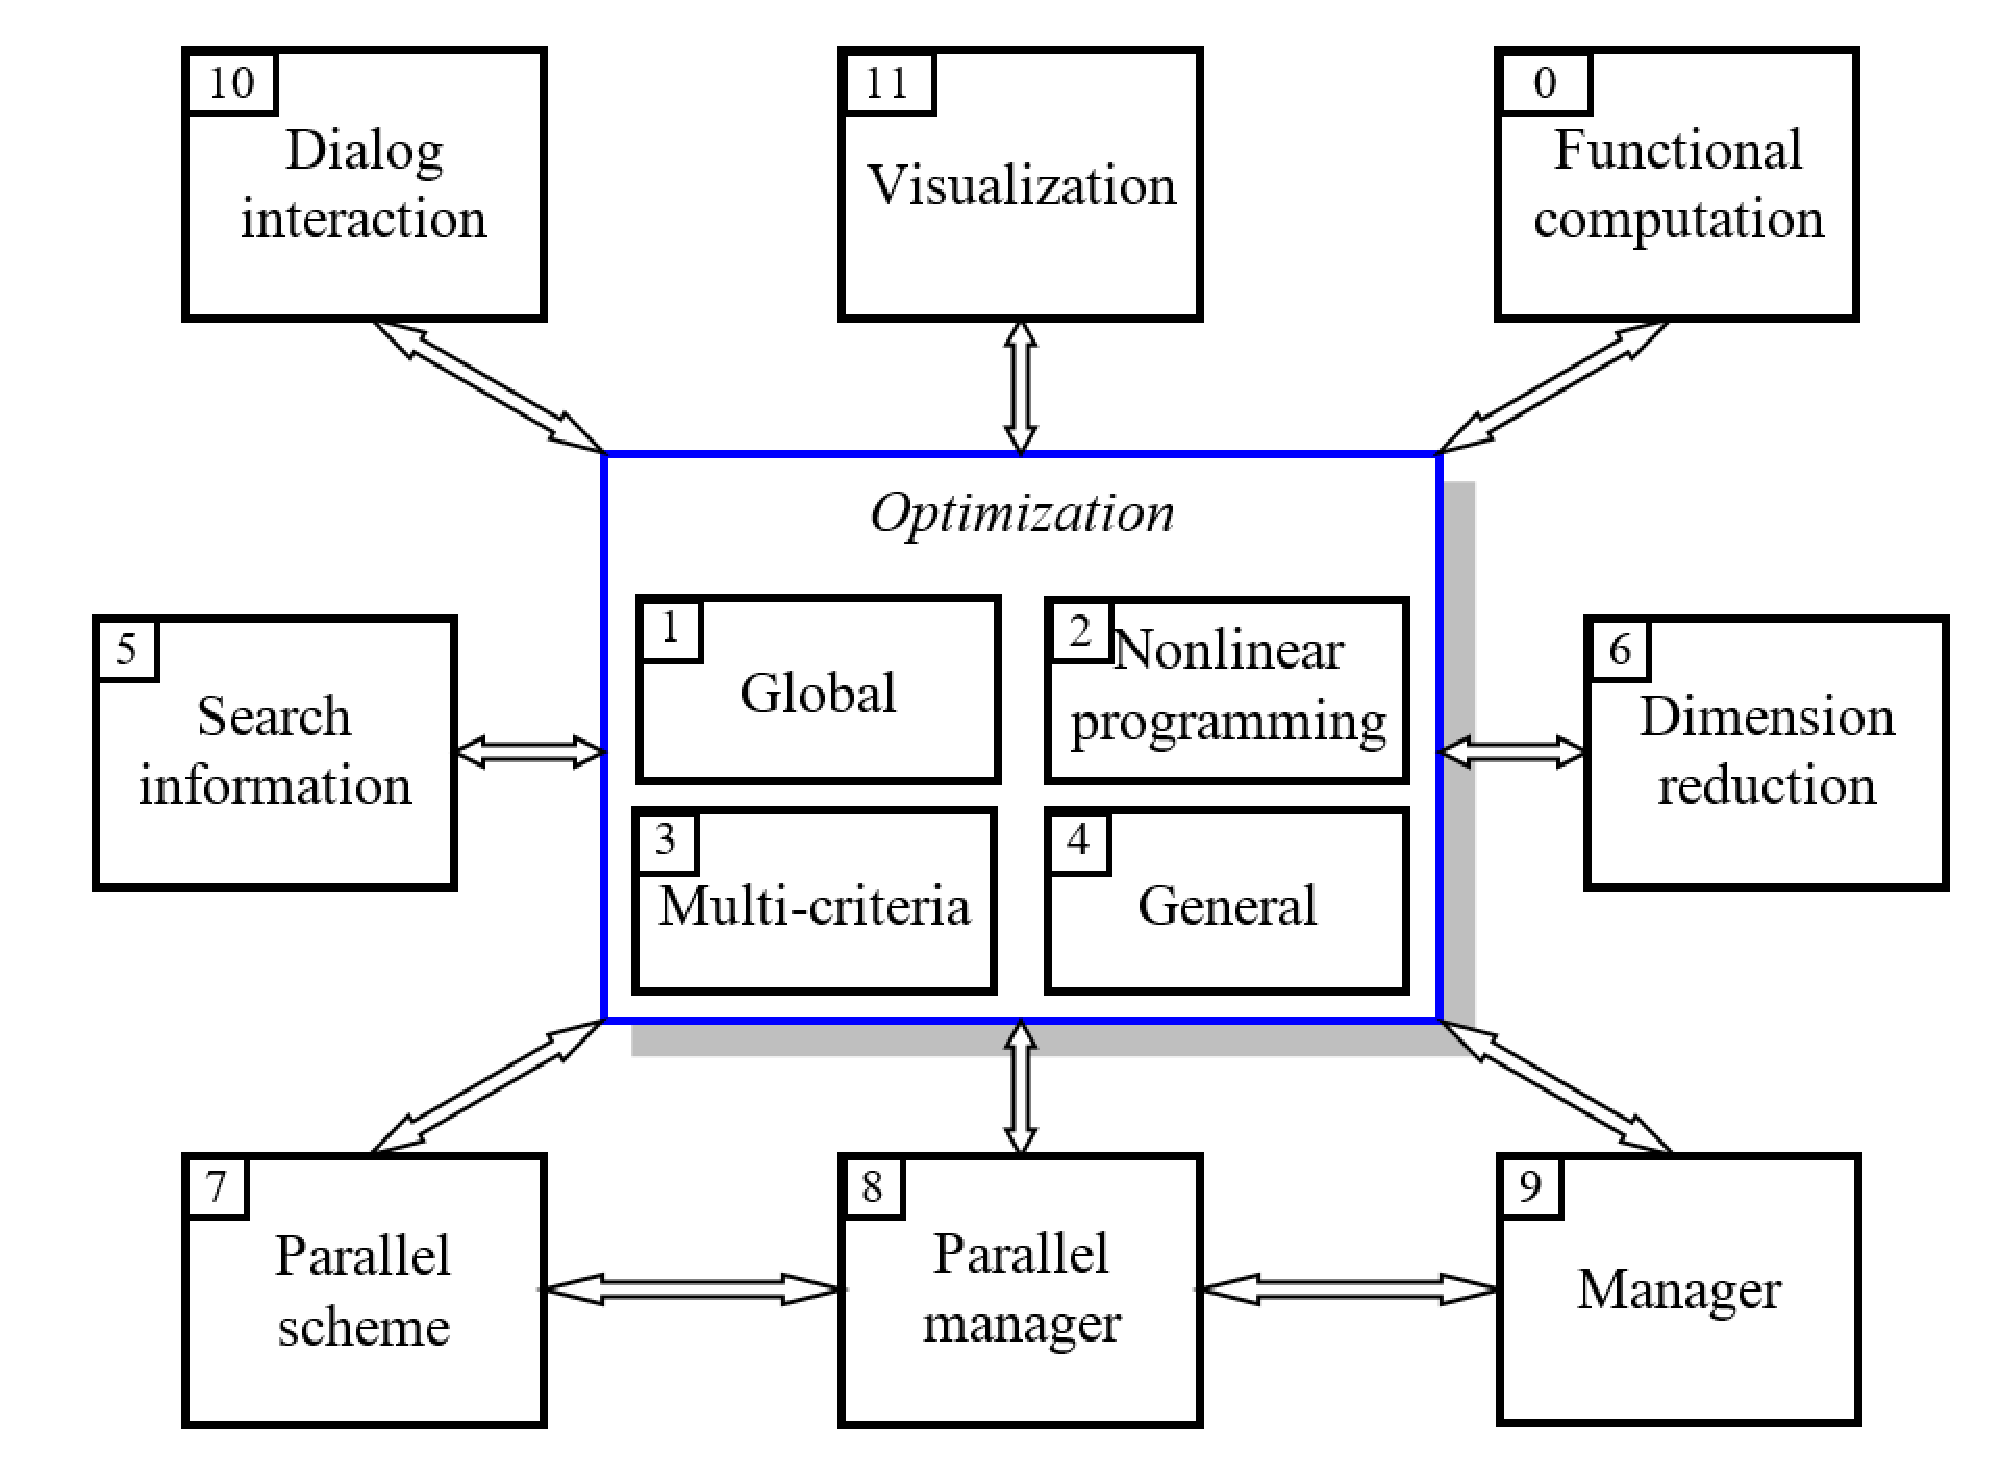
\includegraphics[width=0.75\textwidth]{pictures/globalizerScheme.eps}
		\caption{The Globalizer system architecture (Blocks 1-2, 5-7 have been implemented; Blocks 3-4 and 8-11 are under development)}
    \label{fig:globalizerScheme}
\end{figure}

\par
The Globalizer system architecture is presented in Figure \ref{fig:globalizerScheme}. The structural components are:
\begin{itemize}
  \item Block 0 consists of the procedures for computing the function values (criteria
  and constraints) for the optimization problem being solved; this is an external
  block with respect to the Globalizer system and is provided by the user per a predefined interface.
  \item Blocks 1-4 form the optimization subsystem and solve the global optimization
  problems (Block 1), nonlinear programming (Block 2), multicriterial optimization (Block 3),
  and general decision making problems (Block 4). It is worth noting the sequential
  scheme of interaction between these components --- the decision making problems are
  solved using the multicriterial optimization block, which, in turn, uses the nonlinear programming block, etc.
  \item Block 5 is a subsystem for accumulating and processing the search information;
  this is one of the basic subsystems --- the amount of search information for complex
  optimization problems may appear to be quite large on the one hand, but, on the other
  hand, the efficiency of the global optimization methods depends to a great extent on how
  completely all of the available search data is utilized.
  \item Block 6 contains the dimensional reduction procedures based on Peano evolvents;
  the optimization blocks solve the reduced (one-dimensional) optimization problems;
  Block 6 provides interaction between the optimization blocks and the initial
  multidimensional optimization problem.
  \item Block 7 organizes the choice of parallel computation schemes in the Globalizer
  system subject to the computing system architecture employed (the numbers of cores in the
  processors, the availability of shared and distributed memory, the availability of
  accelerators for computations, etc.) and the global optimization methods applied.
  \item Block 8 is responsible for managing the parallel processes when performing the
  global search (determining the optimal configuration of parallel processes, distributing
  the processes between computer elements, balancing computational loads, etc.).
  \item Block 9 is a common managing subsystem, which fully controls the whole
  computational process when solving global optimization problems.
  \item Block 10 is responsible for organizing the dialog interaction with users for
  stating the optimization problem, adjusting system parameters (if necessary), and
  visualizing and presenting the global search results.
  \item Block 11 is a set of tools for visualizing and presenting the global search results;
  the availability of tools for visually presenting the computational results enables
  the user to provide efficient control over the global optimization process.
\end{itemize}
\par
The Globalizer system comes in two different options:
\begin{itemize}
  \item Globalizer Pro is a research version of the system providing a full set of
  capabilities that are oriented toward solving of the most complicated global optimization problems.
  \item Globalizer Lite is a limited version of the Globalizer system accessible for free for
  solving global optimization problems with a medium level of difficulty, and is accessible free of charge.
\end{itemize}
\section{Results of Numerical Experiments}
\label{sec:experiments}
In order to confirm the operability of the Globalizer system, results from two
series of computational experiments are presented in this section.
\par
The computational experiments were conducted using the Lobachevsky supercomputer at the
State University of Nizhny Novgorod (operation system --- CentOS 6.4, management system --- SLURM).
Each supercomputer node had 2 Intel Sandy Bridge E5-2660 processors, 2.2 GHz, with 64 GB RAM.
Each processor had 8 cores (i.e. a total of 16 CPU cores were available at each node).
In order to generate the executable program code, the Intel C++ 14.0.2 compiler was used.
\par
A number of nodes in the computer system utilized Intel Xeon Phi 5110P processors,
each containing 60 cores (a total of 240 threads). In addition, the supercomputer also
included computer nodes equipped with two GPU NVIDIA Kepler K20Х, each providing 14
stream multiprocessors (a total of 2688 CUDA-cores). In order to generate the executable
code, the CUDA Toolkit 6.0 was used.
\par
The problems generated by the GKLS-generator (Gaviano, M., Lera, D., Kvasov, D. E., Sergeyev, Y. D., 2003)
were selected for the test problems. This generator allowed for obtaining the multiextremal
optimization problems with \textit{a priori} known properties: the number of local minima,
the sizes of their attractors, the global minimum point, the function value at this point, etc.
In order to simulate the computation costs inherent in the applied optimization problems
(see, for example, Bastrakov, S., Gergel, V., Meyerov, I., et al, 2013), in all of the experiments
computing the objective function was complicated by auxiliary computations, not altering the
form of the function and the position of its minima.
\par
We considered the global minimum \(y^*\) in the test problem to be found if the
algorithm generated a trial point \(y^k\) in the \(\delta\)-nearness of the global
minimum i. e. \(\Vert y^k-y^* \Vert \leqslant \delta\). The size of the nearness was
selected as \(\delta=\Vert b-a \Vert\sqrt[N]{\Delta}\) where \(a\) and \(b\) are
boundaries of the search domain \(D\), \(N\) is the dimensionality of the optimization problem.
The maximum allowed number of parallel iterations was \(K_{max} = 10000\), and the evolvent
density parameter was \(m=10\).The computational experiments considered below were first
carried out using the ExaMin system (see (Barkalov, K., Gergel V., 2015), (Barkalov, K., Gergel, V., Lebedev, I., 2015), (Barkalov, K., Gergel, V., Lebedev, I., Sysoev, A., 2015), (Gergel, V., Lebedev, I., 2015))
and then were reproduced using the Globalizer system.

\subsection{Parallel Computations Using Intel Xeon Phi processors}
The results of the numerical experiments with GPMAGS on an Intel Xeon Phi are provided in Table 1.
The computations were performed using the Simple and Hard function classes with the dimensions equal to 4 and 5. The parameters  at  and  at  were used. When using the GPMAGS method, the parameter  was selected for the Simple class, and  was selected for the Hard class.
\par
In the first series of experiments, serial computations using MAGS were executed. The average number of iterations performed by the method for solving a series of problems for each of these classes is shown in row I. The symbol “>” reflects the situation where not all problems of a given class were solved by a given method. It means that the algorithm was stopped once the maximum allowable number of iterations Kmax was achieved. In this case, the Kmax value was used for calculating the average number of iterations corresponding to the lower estimate of this average value. The number of unsolved problems is specified in brackets.
\par
In the second series of experiments, parallel computations were executed on a CPU. The relative “speedup” in iterations achieved is shown in row II; the speedup of parallel computations was measured in relation to the sequential computations (p=1).



\subsection{Parallel Computations Using General Purpose Graphic Processors}

\section{Conclusions}
\label{sec:concl}
In this paper, the Globalizer global optimization software system was examined for
implementing a general scheme for the parallel solution of globally-optimized decision
making using a wide spectrum of computer systems: with shared and distributed memory,
NVIDIA graphic processors and Intel Xeon Phi coprocessors. This approach enables the
efficient use of modern supercomputer systems to solve the most computational costly
multiextremal optimization problems. The computational experiments have confirmed the
prospects for this proposed approach.

\section*{Acknowledgements}
This research was supported by the Russian Science Foundation, project No 16-11-10150
``Novel efficient methods and software tools for time-consuming decision making problems using supercomputers of superior performance.''

\end{document}
